\documentclass[10pt,a4paper]{amsart}
% \usepackage{geometry}\geometry{margin=1.5in}
\usepackage{latexsym, bbm, enumerate, amssymb, amsmath, graphicx, amsthm}
\usepackage{tikz}
% \usepackage[nolists]{endfloat}

\newtheorem{theorem}{Theorem}[section]
\newtheorem{corollary}{Corollary}[theorem]
\newtheorem{lemma}[theorem]{Lemma}
\newtheorem*{remark}{Remark}

% \newcommand{\EE}{{\mathbb{E}}}
\newcommand{\EE}{E}
% \newcommand{\PP}{{\mathbb{P}}}
\newcommand{\PP}{P}
% \newcommand{\E1}{\EE(Y\mid A=1,X)}
% \newcommand{\H}[1]{H^{(1)}_{#1}}
\newcommand{\E}[1]{\EE(Y\mid A=#1,X)}

\DeclareMathOperator{\Var}{Var}
\DeclareMathOperator{\Cov}{Cov}
\DeclareMathOperator{\logit}{logit}
\renewcommand{\includegraphics}[2][]{\fbox{}}

\begin{document}
The data is modeled as:
\begin{gather}
\begin{aligned}
  \label{eqn:model}
  (X_1,Y_1,A_1),\ldots,(X_n,Y_n,A_n) &\overset{iid}{\sim}\mathcal{O}\\
  A&\perp X\\
  \PP(A=1\mid X) = \PP(A=1) = 1-\PP(A=0)&= p
\end{aligned}
\end{gather}
for some law $\mathcal{O}$.
\begin{figure}[h!]
  \centering
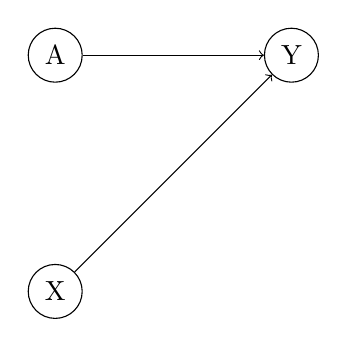
\begin{tikzpicture}
      \node[shape=circle,draw=black] (X) at (0,0) {X};
      \node[shape=circle,draw=black] (A) at (0,3) {A};
      \node[shape=circle,draw=black] (Y) at (3,3) {Y};
      \path [->] (X) edge node[left] {} (Y);
      \path [->] (A) edge node[left] {} (Y);


  \end{tikzpicture}
\end{figure}

The estimand is
$$
\psi_0 = \EE(Y\mid A=1) - \EE(Y\mid A=0).
$$
An estimator is obtained as the solution in $\psi$ of
\[
\sum_{i=1}^nU(Y_i,A_i;\psi) = 0,
\]
where
\[
  U(Y,A;\psi) = (A-p)(Y-\psi A).
\]
Consistency and asymptotic normality of this estimator follow from:
% \footnote{
%   Eric, is this the usual MLE consistency-type argument? Ie, if we can expand in a taylor series
%   about the true parameter,
%   \begin{align*}
%     0 = \sum_i U(X_i,Y_i,A_i; \hat{\psi}) &= \sum_i U(X_i,Y_i,A_i; \psi_0) + (\hat{\psi}-\psi_0)\sum_iU'(X_i,Y_i,A_i; \psi_*)\\
%     n^{1/2}(\hat{\psi}-\psi_0) &= -(n^{-1}\sum_iU'(X_i,Y_i,A_i; \psi_*))^{-1}\times n^{-1/2}\sum_i U(X_i,Y_i,A_i; \psi_0)\\
%     &\leadsto -\EE(U'(X,Y,A;\psi_*))^{-1}\times \mathcal{N}(0,\sigma^2)
%   \end{align*}
%   where use the lemma in concluding that the normal distribution in the
%   last line has mean zero. Implying root-n consistency.
%   }
\begin{lemma}\label{lemma:1}
  $\EE(U(Y,A;\psi_0))=0.$
\end{lemma}
\begin{proof}
  \begin{align*}
    \EE(U(Y,A;\psi_0)) &= \EE[(A-p)(Y-\psi_0 A)]\\
                       &= \EE[(A-p)(\EE(Y\mid A) - \psi_0A)]\\
                       &= (\EE(Y\mid A=1)-\psi_0A)(1-p)p + \EE(Y\mid A=0)(-p)(1-p)\\
                       &= p(1-p)[\EE(Y\mid A=1) - \EE(Y\mid A=0) - \psi_0]=0.
  \end{align*}
\end{proof}

We consider estimators obtained as solutions in $\psi$ to equations of the form
\begin{align}
\sum_iU(Y_i,A_i;\psi) + (A_i-p)h(X_i;\psi)=\sum_i (A_i-p)(Y_i-\psi A_i + h(X_i;\psi))=0\label{eqn:unaugmented}
\end{align}
for [arbitrary] functions $h$. It
follows from Lemma \ref{lemma:1} and (\ref{eqn:model}) that
\[
\EE(U(Y,A;\psi_0) + (A-p)h(X;\psi))=0,
\]
so such estimators are also
asymptotically normal. An additional benefit is that
the asymptotic variance of the resulting estimator may be minimized by
varying $h$, perhaps improving on the efficiency of the estimator obtained
from $\sum_iU(Y,A;\psi)=0$. In fact, the minimizing choice of $h$ is determined
by the estimating equation given by
\begin{align}
  % &= U(Y,A;\psi)-\EE(U(Y,A;\psi)\mid S_A)\nonumber\\
       W(X,Y,A;\psi)      &=U(Y,A;\psi) - \EE(U(Y,A;\psi)\mid A,X) + \EE(U(Y,A;\psi)\mid X).\label{eqn:augmented}
\end{align}
A proof is given in Lemma \ref{lemma:min_h}, after rewriting the rhs
of (\ref{eqn:augmented}), as follows. The middle term on the rhs of (\ref{eqn:augmented}) is,

\begin{align*}
  \EE(U(Y,A;\psi)\mid A,X) &= \EE((A-p)(Y-\psi A)\mid A,X)\\
                           &= (\EE(Y\mid A,X)-\psi A)(A-p)\\
                           &=[\EE(Y\mid A=1,X)A + \EE(Y\mid A=0,X)(1-A)](A-p) - \psi A(A-p)\\
                           &= \EE(Y\mid A=1,X)A(1-p) - \EE(Y\mid A=0,X)(1-A)p - \psi A(1-p).
\end{align*}
The last term on the rhs of (\ref{eqn:augmented}) is then,
\begin{align*}
  \EE(U(Y,A;\psi)\mid X) &= p  \EE(U(Y,A;\psi)\mid A=1,X) + (1-p)  \EE(U(Y,A;\psi)\mid A=0,X)\\
                         &= p[\EE(Y\mid A=1,X)(1-p) - \psi (1-p)] - (1-p)[\EE(Y\mid A=0,X)p]\\
                         &= p(1-p)(\EE(Y\mid A=1,X) - \EE(Y\mid A=0,X) - \psi).
\end{align*}
Therefore,
\begin{align*}
  W(X,Y,A;\psi) &= U(Y,A;\psi) - \EE(U(Y,A;\psi)\mid A,X) + \EE(U(Y,A;\psi)\mid X)\\
                &= (A-p)(Y-\psi A) - (A-p)(1-p)\EE(Y\mid A=1,X) - (A-p) p\EE(Y\mid A=0,X) + \\
                &\qquad (A-p)(1-p)\psi\\
                &= (A-p)[Y - (1-p)\EE(Y\mid A=1,X) - p\EE(Y\mid A=0,X)] - p(1-p)\psi\\
% \end{align*}
% From the relations
% \begin{equation}
%   \begin{aligned}
%     \label{eqn:relations}
%   \EE(Y\mid X) &= p\E1 + (1-p)\E0\\
%   \E1 &= A\E1 = (A/p)[E(Y\mid X) - (1-p)\E0]\\
%   &=(A/p)\EE(Y\mid X)\\
%   \E0 &= (1-A)\E0 = [(1-A)/(1-p)][E(Y\mid X) - p\E1]\\
%   &=[(1-A)/(1-p)]\EE(Y\mid X),
% \end{aligned}
% \end{equation}
% we re-write $W(X,Y,A;\psi)$ so as to avoid the regressions on the
% treatment levels:
% \begin{align*}
%   W(X,Y,A;\psi) &= (A-p)[Y - (1-p)\E1 - p\E0] - p(1-p)\psi\\
%                 &= (A-p)[Y - (A(1-p)/p + (1-A)p/(1-p))\EE(Y\mid X)] - p(1-p)\psi\\
%                 &= (A-p)[Y - \frac{(A-p)^2}{p(1-p)}\EE(Y\mid X)] - p(1-p)\psi.
% \end{align*}
&= (A-p)[Y - \EE(\tilde{Y}\mid X)] - p(1-p)\psi\\
                &= U(Y_i,A_i;\psi) + (A-p)[\psi A - \EE(\tilde{Y}\mid X)] - p(1-p)\psi,
\end{align*}
where $\tilde{Y}$ is determined by the transformation
\[
  Y = \tilde{Y}\frac{p^A(1-p)^{1-A}}{(1-p)^Ap^{1-A}}=\tilde{Y}\left(\frac{p}{1-p}\right)^{2A-1}.
\]
In case $p=\PP(A=1)=\PP(A=0)=1/2,$
\begin{align}
  W(X,Y,A;\psi) = (A-1/2)(Y-\EE(Y\mid X)) - \psi/4.\label{eqn:W_basic}
\end{align}
% The first term on the rhs of (\ref{eqn:augmented}) is
% \begin{align*}
    %     \EE(U(\psi)\mid A,X) &= (\EE(Y\mid A,X)-\psi A)(-1)^{1-A}\\
    %                                &= A[\EE(Y\mid A=1,X) - \psi + \EE(Y\mid A=0,X)] - \EE(Y\mid A=0,X).
% \end{align*}
% For the second equality we use the identity $g(a,x)=a[g(1,x)-g(0,x)] +
% g(0,x),$ which holds for $a\in\{0,1\}$ and arbitrary $g,x,$ applied to the function
% $g:(a,x)\mapsto(\EE(Y\mid a,x)-\psi a)(-1)^{1-a}.$ The second term on
% the rhs of (\ref{eqn:augmented}) is
% \begin{align*}
%   \EE(U(\psi)\mid X) &= (1/2)[\EE(U(\psi)\mid A=1,X) + \EE(U(\psi)\mid A=0,X)]\\
%                      &= (1/2)[\EE(Y\mid A=1,X) - \psi - \EE(Y\mid A=0,X)],
% \end{align*}
% using in the first equality that $A$ and $X$ are independent under
% (\ref{eqn:model}). Combining the last two displays,
% \begin{align*}
%   W(\psi) &:= U(\psi) - \EE(U(\psi)\mid A,X) + \EE(U(\psi)\mid X)\\
%           &= U(\psi) - (A-1/2)[\EE(Y\mid A=1,X) + \EE(Y\mid A=0,X) - \psi]\\
%           &= U(\psi) - (A-1/2)[2\EE(Y\mid X) - \psi].
% \end{align*}

\begin{lemma}\label{lemma:min_h}
  The asymptotic variance of the estimator obtained as the solution in $\psi$ to
  \begin{align}
    \sum_iU(Y_i,A_i;\psi) + (A_i-p)h(X_i;\psi)=\sum_i (A_i-p)(Y_i-\psi A_i + h(X_i;\psi))=0\label{eqn:min_h}
  \end{align}
  is minimized over arbitrary functions $h$ of $X$ at
  \[ h_0(X;\psi)=(A-p)[\psi A - \EE(\tilde{Y}\mid X)] - p(1-p)\psi.\]

\end{lemma}

\begin{proof}
  We give the $p=\PP(A=1)=1/2$ case, in which case
  \[ h_0(X;\psi)=(A-1/2)[\psi A-\EE(Y\mid X)]-\psi/4.\]
  Under suitable regularity conditions, the asymptotic
  variance of the solution to the estimating equation
  (\ref{eqn:min_h}) is given by the variance of its influence
  function. Since
  \[ \EE \frac{\partial}{\partial\psi}[U(Y_i,A_i;\psi) + (A_i-p)h(X_i;\psi)]=\EE \frac{\partial}{\partial\psi}U(Y_i,A_i;\psi),
  \]
  the influence function of (\ref{eqn:min_h}) is
  \[
  -\left(\EE\left.\frac{\partial}{\partial\psi}U(Y,A;\psi) \right\vert_{\psi_0}\right)^{-1}(U(Y,A;\psi_0)+(A-1/2)h(X;\psi)).
\]
Thus we wish to show
\begin{align*}
  \Var\left[\left(\EE\frac{\partial}{\partial\psi}U(Y,A;\psi_0)\right)^{-1}(U(Y,A;\psi_0)+(A-1/2)h(X;\psi))\right]\ge\\
   \Var\left[\left(\EE\frac{\partial}{\partial\psi}U(Y,A;\psi_0)\right)^{-1}(U(Y,A;\psi_0)+(A-1/2)h_0(X;\psi))\right]
\end{align*}
or
\begin{gather}
\begin{aligned}\label{lemma:min_h:step_1}
  \EE[(A-1/2)^2h^2(X)] + 2\EE[U(Y,A;\psi_0)(A-1/2)h(X;\psi)] \ge\\
  \EE[(A-1/2)^2h_0^2(X)] + 2\EE[U(Y,A;\psi_0)(A-1/2)h_0(X;\psi)].
\end{aligned}
\end{gather}
Since $A,X$ are uncorrelated, and noting that $(A-1/2)(-1)^{1-A}=1/2,$ the lhs is
\begin{align*}
  &\EE[(A-1/2)^2h^2(X)] + 2\EE[U(Y,A;\psi_0)(A-1/2)h(X;\psi)]\\
  &=\Var(A)\EE h^2(X) + 2\EE[(A-1/2)\EE(U(Y,A;\psi_0)h(X;\psi)\mid A)]\\
  &= \EE h^2(X)/4 + 2\EE[(A-1/2)\EE((Y-\psi_0 A)(-1)^{1-A}h(X;\psi)\mid A)]\\
  &= \EE h^2(X)/4 + \EE[\EE((Y-\psi_0 A)h(X;\psi)\mid A)]\\
    &= \EE h^2(X)/4 + \EE((Y-\psi_0/2)h(X;\psi)).
\end{align*}
We obtain an expression for the rhs by substituting $h(X;\psi):=h_0(X;\psi)=-(2\EE(Y\mid
X)-\psi_0),$
\begin{align*}
  &\EE[(A-1/2)^2h_0^2(X)] + 2\EE[U(Y,A;\psi_0)(A-1/2)h_0(X;\psi)]\\
  &= \EE h_0^2(X)/4 + \EE((Y-\psi_0/2)h_0(X;\psi))\\
  &= \EE[h_0(X;\psi)(h_0(X;\psi)/4 + Y - \psi_0/2)]\\
  &= \EE[h_0(X;\psi)(-(2\EE(Y\mid X)-\psi_0)/4 + E(Y\mid X) - \psi_0/2)]\\
  &= \EE[h_0(X;\psi)(E(Y\mid X)/2 - \psi_0/4)]\\
  &= -\EE h_0^2(X)/4 \addtocounter{equation}{1}\tag{\theequation}\label{eqn:decrement}\\
  &= -\EE[\EE(Y\mid X)^2] + \psi_0\EE Y - \psi_0^2/4.
\end{align*}
Thus (\ref{lemma:min_h:step_1}), which we wish to show, becomes
\begin{align*}
  \EE h^2(X)/4 + \EE((Y-\psi_0/2)h(X;\psi)) + \EE[\EE(Y\mid X)^2] - \psi_0\EE Y + \psi_0^2/4 \ge 0.
\end{align*}
This inequality follows by an application of the Cauchy-Schwarz inequality,
\begin{align*}
  &\EE h^2(X)/4 + \EE((Y-\psi_0/2)h(X;\psi)) + \EE[\EE(Y\mid X)^2] - \psi_0\EE Y + \psi_0^2/4 \\
  &= (1/4)\EE[(h(X;\psi)-\psi_0)^2] + \EE(Yh(X;\psi)) + \EE[\EE(Y\mid X)^2] - \psi_0\EE Y\\
  % &= (1/4)\EE[(h(X;\psi)-\psi_0)^2] + \EE[\EE(Y\mid X)^2] + \EE[Y(h(X;\psi)-\psi_0)]\\
  &= (1/4)\EE[(h(X;\psi)-\psi_0)^2] + \EE[\EE(Y\mid X)^2] + \EE[\EE(Y\mid X)(h(X;\psi)-\psi_0)]\\
  &\ge (1/4)\EE[(h(X;\psi)-\psi_0)^2] + \EE[\EE(Y\mid X)^2] - \EE[(h(X;\psi)-\psi_0)^2]^{1/2}\EE[\EE(Y\mid X)^2]^{1/2}\\
  &= \{(1/2)\EE[(h(X;\psi)-\psi_0)^2]^{1/2} - \EE[\EE(Y\mid X)^2]^{1/2} \}^2 \ge 0.
\end{align*}
\end{proof}

\begin{remark}
From (\ref{eqn:decrement}), $\EE h_0^2(X)/4$ is the reduction in the
asymptotic variance gained by
using (\ref{eqn:min_h}) over (\ref{eqn:unaugmented}).
\end{remark}

% From the identity $(-1)^{1-a}=(2a-1)=2(a-1/2), a\in\{0,1\},$ we
% write
% $$
% U(\psi)=(Y-\psi A)(-1)^{1-A}=2(A-1/2)(Y-\psi A),
% $$
% obtaining
% \begin{align*}
%   W(\psi) &= U(\psi) - (A-1/2)[2\EE(Y\mid X) - \psi]\\
%           &= (A-1/2)[2(Y-\EE(Y\mid X))-\psi(2A-1)]\\
%           &= (A-1/2)[2(Y-\EE(Y\mid X))+(-1)^A\psi].
% \end{align*}

% [[Extension to $\PP(A=1\mid X)=p\in(0,1)$]]

The expression for $W(X,Y,A;\psi)$ in (\ref{eqn:augmented}) contains a term
of the form $E(Y\mid A,X),$ generally requiring estimation, whereas the equivalent expression in
(\ref{eqn:W_basic}) only requires $E(Y\mid X)$ to be estimated. We
investigate whether the second form is more resistant to bias by an
unscrupulous analyst.

% Suppose data is generated under the following mechanism, consistent
% with (\ref{eqn:model}):
% \[\]
Consider the following strategies for estimating $\psi$:
\begin{enumerate}
\item \label{item:nonblinded} The analyst first forms $2^{p+1}$
  estimates of $E(Y\mid A,X)$ by fitting submodels of the linear model
  \[E(Y\mid A,X) = A + X_1 + \ldots + X_p + \text{second-order interactions}.\]
  For each estimate $E(Y\mid A,X)$, the analyst
  then obtains an estimate for $\psi$ by solving the estimating equation (\ref{eqn:augmented}),
  using the model estimate of $E(Y\mid A_i,X_i), i=1,\ldots,n.$ From
  the resulting estimates for $\psi,$ the analyst reports the
  largest.
\item \label{item:blinded} One analyst is given the control data
  \[\{(Y_i,X_i) : A_i=0\}\]
  from which he forms estimates of $E(Y\mid A=0, X)$ using submodels
  of the linear models
\[E(Y\mid X) = X_1 + \ldots + X_p + \text{second-order
    interactions}.\]
Another analyst estimates $E(Y\mid A=1,X)$ analogously. The models
  are combined to estimate $E(Y\mid A,X)$ and obtain estimates of
  $\psi$ as before, from which the largest is chosen.
\item \label{item:ours} The analyst proceeds as in (\ref{item:nonblinded}), but omitting $A_i$
  from his models. I.e., the analyst first forms
  estimates of $E(Y\mid X)$ by fitting submodels of the linear model
  \[E(Y\mid X) = X_1 + \ldots + X_p + \text{second-order interactions}.\]
  For each estimate $E(Y\mid X)$, the analyst
  then obtains an estimate for $\psi$ by solving the estimating equation (\ref{eqn:W_basic}),
  using the model estimate of $E(Y\mid X_i), i=1,\ldots,n.$ From
  the resulting estimates for $\psi,$ the analyst reports the
  largest.
  \item \emph{Not yet done.} As in (\ref{item:blinded}), two analysts each obtain $2^p$
    estimates of $E(Y\mid
    A=1,X)$ and $E(Y\mid A=1,X)$ separately, but now the maximum estimate
    of $\psi$ is obtained ranging over all $2^{p+1}$ pairs of the 2
    analysts' sets of estimates.
\end{enumerate}

The results of a simulation are in Figure \ref{fig:1}. From the
simulation, the reported $\psi$ estimates are less biased when computed
under method (\ref{item:ours}) and (\ref{item:blinded}) than method (\ref{item:nonblinded}), though all methods are seriously biased. Also plotted is the average, rather than maximum
$\psi$ estimate, over the sets of models considered under each
method. These are close to the true value $\psi=1,$ particularly for
larger $n,$ as expected.

Since all methods are so biased, confidence intervals at this range of
sample sizes ($\le 300$) are useless. Increasing the sample size to
1000 allows some comparison of error rates. Figure \ref{fig:2} gives
the coverage rates of the 3 methods for as the number of covariates
given to the analysts ranges.

\begin{figure}
  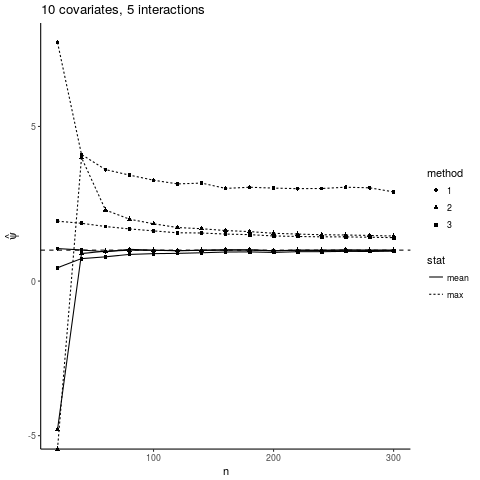
\includegraphics[width=\linewidth]{171006a.png}
  \caption{Comparison of the 3 methods of estimating $\psi$.}  \label{fig:1}

\end{figure}


\begin{figure}
  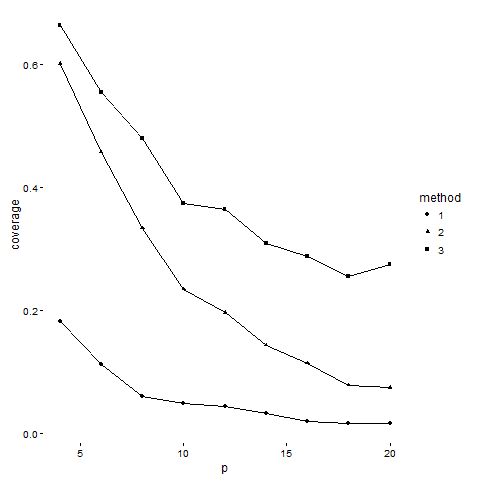
\includegraphics[width=\linewidth]{171017.png}
  \caption{Coverage rates of 3 $\psi$ estimates when the sample size
    is $n=1000$.}  \label{fig:2}
\end{figure}

\subsection{Equivalence to regression estimator}

Define
\[
  \tilde{Y} = Y - \EE(Y\mid X)
\]
and consider the regression
\[
  \EE(\tilde{Y} \mid A) = \beta_0 + \beta_1A.
\]
Then $\beta_0 + \beta_1 = \EE(\tilde{Y}\mid A=1) = \EE(Y\mid A=1) -
E(Y)$ and $\beta_0 = \EE(\tilde{Y}\mid A=0) = \EE(Y\mid A=0) -
E(Y) = \EE(Y\mid A=0)/2 - \EE(Y\mid A=1)/2,$ so
\begin{align*}
  \beta_0 &= -\psi/2\\
  \beta_1 &= \psi.
\end{align*}

The influence function of $(\beta_0,\beta_1)$ is obtained as:
\begin{align*}
  0 &= \sum_{i=1}^n\begin{pmatrix}1\\A_i\end{pmatrix}(\tilde{Y}_i - \hat{\beta_0} - A_i\hat{\beta_1})\\
    &= \sum_{i=1}^n\left\{\begin{pmatrix}1\\A_i\end{pmatrix}(\tilde{Y}_i - \beta_0 - A_i\beta_1) +
  \begin{pmatrix}-1&-A_i\\-A_i&-A_i\end{pmatrix}\begin{pmatrix}\hat{\beta_0}-\beta_0\\ \hat{\beta_1}-\beta_1\end{pmatrix}\right\}\\
  n^{1/2}\begin{pmatrix}\hat{\beta_0}-\beta_0\\ \hat{\beta_1}-\beta_1\end{pmatrix} &=\left(\frac{1}{n}\sum_i\begin{pmatrix}1&A_i\\A_i&A_i\end{pmatrix}\right)^{-1}n^{-1/2}\sum_i \begin{pmatrix}1\\A_i\end{pmatrix}(\tilde{Y}_i - \beta_0 - A_i\beta_1)\\
    &=\begin{pmatrix}1&1/2\\1/2&1/2\end{pmatrix}^{-1}n^{-1/2}\sum_i \begin{pmatrix}1\\A_i\end{pmatrix}(\tilde{Y}_i - \beta_0 - A_i\beta_1)+o_P(1)\\
  n^{1/2}(\hat{\beta}_1 - \beta_1) &= n^{-1/2}\sum_i \begin{pmatrix}-2 & 4\end{pmatrix}\begin{pmatrix}1\\A_i\end{pmatrix}(\tilde{Y}_i - \beta_0 - A_i\beta_1) + o_P(1)\\
    &= 4n^{-1/2}\sum_i (A_i-1/2)(\tilde{Y}_i - \beta_0 - A_i\beta_1) + o_P(1)\\
    &= 4n^{-1/2}\sum_i (A_i-1/2)(\tilde{Y}_i - (A_i - 1/2)\psi) + o_P(1)\\
    &= 4n^{-1/2}\sum_i \left\{(A_i-1/2)(Y-\EE(Y\mid X)) - \psi/4\right\} + o_P(1).
\end{align*}
By comparison with (\ref{eqn:W_basic}), we find that $\hat{\psi},$ the
augmented estimator, is asymptotically equivalent to $\hat{\beta_1}.$

On the other hand, the OLS solution to the above regression gives
\[
  \hat{\beta_1} = \hat{\Cov}(\tilde{Y},A)/\hat{\Var}(A) = \frac{\overline{A\tilde{Y}}/\bar{\tilde{Y}} - \bar{\tilde{Y}}}{1-\bar{A}}
\]
whereas from (\ref{eqn:W_basic}),
\[
  \hat{\psi}=\bar{\tilde{Y}}/2 - \overline{A\tilde{Y}},
\]
so the two estimators are not equal.
\section{Other estimands}
As above, the full data is $Y_i^*=(Y_i^*(0),Y_i^*(1)),i=1,\ldots,n,$ the observed data is $(Y_i,A_i,X_i),i=1,\ldots,n,$ and we assume
\begin{align*}
  &Y = AY^*(1) + (1-A)Y^*(0),\\
  &\PP(A=1)=p\in (0,1)\\
  &A \perp X, A\perp Y^*.
\end{align*}
Besides the mean treatment difference $\EE(Y\mid A=1) -
\EE(Y\mid A=0)$ discussed above, we consider other estimands:
\begin{enumerate}
\item $\psi_0 = \log\frac{E(Y^*(1))}{E(Y^*(0))}=\log\frac{E(Y\mid A=1)}{E(Y\mid
    A=0)}$
\item the slope in the model
  \[
    \logit(A\EE(Y^*(1)) + (1-A)\EE(Y^*(0))) = \logit(P(Y=1\mid A))
    = \psi_0 + \psi_1A,
  \]
  for a binary-valued response $Y$
\end{enumerate}

In each case, we obtain the efficient augmented influence function
following the approach of [[Tsiatis ch. 13]]:
\begin{enumerate}
\item obtain a full-data influence function $\phi^F(Y^*)$
  \item obtain an observed data influence function $\phi(Y,A,X)$ corresponding to
    $\phi^F$ under the mapping $\phi \mapsto \EE(\phi\mid Y^*)$
  \item compute the efficient augmentation term
    \begin{align*}
      h^*(Y,A,X)&=(A-p)(\EE(\phi\mid A=1,X) - \EE(\phi\mid A=0,X))\\
                &=\EE(\phi\mid A,X) - \EE(\phi\mid X)
    \end{align*}

\end{enumerate}
We then eliminate regressions on treatment level, i.e., the terms $\EE(Y\mid A=1,X)$ and
$\EE(Y\mid A=0,X).$

% \subsection{$\EE\left(\log\frac{Y^*(1)}{Y^*(0)}\right)$}
% The problem is to estimate
% \[
%   \psi_1 = \EE\left(\log\frac{Y^*(1)}{Y^*(0)}\right),
% \]

% An estimator using the full data $Y_i^*=(Y^*_i(0),Y^*_i(1)),i=1,\ldots,n,$ is
% \[
%   n^{-1}\sum_i \EE\left(\log\frac{Y^*_i(1)}{Y^*_i(0)}\right),
% \]

% with influence function

% \[
%   \phi^F(Y^*)= \log\frac{Y^*_i(1)}{Y^*_i(0)} - \psi_1.
% \]

% This is the only influence function [[ref]], so influence functions
% based on the observed data are of the form
% \begin{align}
%   \{\phi(Y,A,X) + h(Y,A,X) : \EE(h(Y,A,X)\mid Y^*)=0\}\label
%   {eqn:logodds_general}
% \end{align}
% with $\phi$ any particular function of the observed data such that
% \[
%   \EE(\phi(Y,A,X)\mid Y^*) = \phi^F(Y^*).
% \]
% An example of such a function is $\phi(Y,A,X)=\frac{A-p}{p(1-p)}\log Y-\psi_1:$
% \begin{align*}
%   \EE((A-p)\log Y\mid Y^*) &= p(1-p)\EE(\log Y\mid Y^*,A=1) - (1-p)p\EE(\log Y\mid Y^*,A=0)\\
%                            &=p(1-p)\left( \EE(\log Y^*(1)\mid Y^*,A=1) - \EE(\log Y^*(0)\mid Y^*,A=0)\right)\\
%                            &= p(1-p)\log\frac{Y^*(1)}{Y^*(0)},\\
%   \EE(\phi(Y,A,X)\mid Y^*)&=\EE\left(\frac{A-p}{p(1-p)}\log Y-\psi_1\mid Y^*\right)\\
%                            &=\log\frac{Y^*(1)}{Y^*(0)} - \psi_1=\phi^F(Y^*).
% \end{align*}
% The variance of an influence of the form given by
% (\ref{eqn:logodds_general}) is minimized for the choice of $h$ given
% by
% \begin{align*}
%   h^*(Y,A,X) &=(A-p)(\EE(\phi\mid A=1,X) - \EE(\phi\mid A=0,X))\\
%            &=\frac{A-p}{p(1-p)}(\EE((A-p)\log Y\mid A=1,X) - \EE((A-p)\log Y\mid A=0,X))\\
%            &=\frac{A-p}{p(1-p)}((1-p)\EE(\log Y\mid A=1,X) + p\EE(\log Y\mid A=0,X)).
% \end{align*}
% The first equality is proven in [[Tsiatis ch.13]].
% The efficient influence function is therefore
% \begin{align*}
%   \phi^*(Y,A,X;\psi_1)&= \phi(Y,A,X;\psi_1) - h^*(Y,A,X)\\
%                  &= \frac{A-p}{p(1-p)}(\log Y - (1-p)\EE(\log Y\mid A=1,X) - p\EE(\log Y\mid A=0,X)) - \psi_1.
% \end{align*}
% In case $p=1-p=1/2,$
% \begin{align*}
%   \phi^*(Y,A,X;\psi_1) = 4(A-1/2)(\log Y - \EE(\log Y\mid X)) - \psi_1,
% \end{align*}
% only requiring $\EE(\log Y\mid X)$ to be estimated. For general $p$, by
% taking
% \[
%   \tilde{Y} = Y^{\frac{p}{1-p}^{2A-1}},
% \]
% we may write
% \[
%   \phi^*(Y,A,X;\psi_1) = 4(A-1/2)(\log \tilde{Y} - \EE(\log Y\mid X)) - \psi_1.
% \]
\subsection{$\log\frac{E(Y\mid A=1)}{E(Y\mid  A=0)}$} The problem is to
estimate
\[
  \psi_0 = \log\frac{E(Y^*(1))}{E(Y^*(0))}=\log\frac{\EE(Y\mid A=1)}{\EE(Y\mid A=0)}.
\]
A full-data estimator is given by the solution to
\[
  \sum_i (Y_i^*(1)-e^{\psi_0}Y_i^*(0))=0,
\]
with influence function
\begin{align*}
  \phi^F(Y,A,X;\psi) &= (e^{\psi}\EE(Y^*
                       (0)))^{-1}   (Y^*(1)-e^{\psi}Y^*(0))\\
                     &= (\EE(Y^*(1)))^{-1}   (Y^*(1)-e^{\psi}Y^*(0)).
\end{align*}
An influence functions $\phi$ of the observed data satisfies
\begin{align*}
  \EE(Y^*_i(1))\phi(Y,A,X) &= \left(\frac{A}{p} - e^{\psi_0}\frac{1-A}{1-p}\right)Y + h(Y,A,X)\\
              &= (A-p)\left(\frac{A}{(A-p)p} - e^{\psi_0}\frac{1-A}{(A-p)(1-p)}\right)Y + h(Y,A,X)\\
              &= \frac{A-p}{p(1-p)}(A + e^{\psi_0}(1-A))Y + h(Y,A,X)\\
              &= \frac{A-p}{p(1-p)}e^{(1-A)\psi_0}Y + h(Y,A,X),
\end{align*}
where $h$ satisfies $\EE(h(Y,A,X)\mid Y^*) = 0.$ The minimizing $h$ is given by
subtracting out
\begin{align*}
  h^*(Y,A,X) &= (A-p)[\EE(\frac{A-p}{p(1-p)}e^{(1-A)\psi_0}Y\mid A=1,X) - \EE(\frac{A-p}{p(1-p)}e^{(1-A)\psi_0}Y\mid A=0,X)]\\
             &= (A-p)[\frac{1}{p}\E1 + \frac{e^{\psi_0}}{1-p}\E0].
\end{align*}
The efficient influence function is therefore
\begin{align*}
  \phi^*(Y,A,X) &= (\EE(Y^*(1)))^{-1} \phi(Y,A,X) - h^*(Y,A,X)\\
                &= (\EE(Y^*(1)))^{-1} (A-p)\left(\frac{e^{(1-A)\psi_0}}{p(1-p)}Y - \frac{1}{p}\E1 - \frac{e^{\psi_0}}{1-p}\E0\right).
\end{align*}
Let $\hat{\psi}_n$ be a consistent estimator of $\psi_0$. Under the transformation
\[
  Y = \frac{p^{2A}(1-p)^{2(1-A)}}{e^{(1-A)\hat{\psi}_n}}\tilde{Y}
\]
the efficient influence function may be rewritten
\begin{align*}
  \phi^*(Y,A,X) &= (\EE(Y^*(1)))^{-1}(A-p)\left(\frac{e^{(1-A)\psi}}{p(1-p)} Y - \EE(\tilde{Y}\mid X)\right) + o_P(1).
                % &= (A-p)\left(\frac{(A + e^{\psi}(1-A))}{p(1-p)} \frac{p^{2A}(1-p)^{2(1-A)}}{e^{(1-A)\psi}}\tilde{Y} - \EE(\tilde{Y}\mid X)\right) + o_P(1).
                % &= (A-p)\left(\left(\frac{Ap}{1-p} + \frac{(1-A)(1-p)}{p}\right)\tilde{Y} - \EE(\tilde{Y}\mid X)\right) + o_P(1)\\
                % &= (A-p)\left(\frac{(1-p)^2-A(1-2p)}{p(1-p)}\tilde{Y} - \EE(\tilde{Y}\mid X)\right) + o_P(1)\\
                % &= (A-p)\left(\left(\frac{p}{1-p}\right)^{2A-1}\tilde{Y} - \EE(\tilde{Y}\mid X)\right) + o_P(1).
\end{align*}
In case $p=1/2,$ $\tilde{Y}=4e^{(1-A)\hat{\psi}_n}Y,$ and
\begin{align}
  \phi^*(Y,A,X) = 2(\EE(Y^*(1)))^{-1}(2A-1)[e^{(1-A)\psi}Y - \EE(e^{(1-A)\hat{\psi}_n}Y\mid X)] + o_P(1).\label{fla:inf_2_simple}
\end{align}

\subsubsection{Two-step regression}
Let
\[
  Z = Y - e^{(A-1)\psi_0}[\EE(e^{(1-A)\psi_0}Y\mid X) - \EE(Y\mid A=1)]
\]
and consider the log-linear regression model
\begin{align}
  \log(\EE(Z\mid A)) = \beta_0 + \beta_1A.\label{model:loglinear}
\end{align}

Then
\[
  \EE(e^{(1-A)\psi_0}Y) = (1/2)[e^{\psi_0}\EE(Y\mid A=0) + \EE(Y\mid A=1)] = \EE(Y\mid A=1)
\]
implies
\begin{align*}
  \EE(Z\mid A=1) &= \EE(Y\mid A=1) - \EE[\EE(e^{(1-A)\psi_0}Y\mid X) - \EE(Y\mid A=1) \mid A=1]\\
                 &= \EE(Y\mid A=1) - \EE(e^{(1-A)\psi_0}Y) + \EE(Y\mid A=1)\\
                 &= \EE(Y\mid A=1),
\end{align*}
and similarly
\begin{align*}
  \EE(Z\mid A=0) &= \EE(Y\mid A=0) - \EE[\EE(e^{(1-A)\psi_0}Y\mid X) - \EE(Y\mid A=1) \mid A=0]\\
                 &= \EE(Y\mid A=0).
\end{align*}
Therefore, under model (\ref{model:loglinear}),
\begin{align*}
  \beta_0 &= \log(\EE(Z\mid A = 0)) = \log(\EE(Y\mid A = 0)),\\
  \beta_0 + \beta_1 &= \log(\EE(Z\mid A = 1)) = \log(\EE(Y\mid A = 1
                      )),\\
  \beta_1 &= \frac{\log(\EE(Y\mid A = 1))}{\log(\EE(Y\mid A = 0))} = \psi_0.
\end{align*}
An estimator $(\hat{\beta}_0, \hat{\beta}_1)$ under the log-linear
regression model (\ref{model:loglinear}) is given by the estimating equations
\[
  0 = \sum_{i=1}^n \begin{pmatrix} 1 \\ A_i \end{pmatrix}(Z_i - e^{\hat{\beta}_0 + \hat{\beta}_1}).
\]
The influence function of $\beta_1=\psi_0$ is computed to be
\begin{align*}
  \phi_{\beta_1}(Y,A,X;\beta) &= 2(2A-1)(e^{-\beta_0-\beta_1A}Z - 1)\\
                    &= 2(2A-1)\left(\frac{Z}{\EE(Z\mid A)} - 1\right)\\
                    &= 2(2A-1)\left(\frac{e^{(1-A)\beta_1}Z}{\EE(Z\mid A=1)} - 1\right)\\
                    % &= 2(2A-1)\frac{e^{(1-A)\beta_1}Z - \EE(Z\mid A=1)}{\EE(Z\mid A=1)}\\
                    &= 2(2A-1)\frac{e^{(1-A)\beta_1}Y - \EE(e^{(1-A)\psi_0}Y\mid X) + \EE(Y\mid A=1) - \EE(Z\mid A=1)}{\EE(Z\mid A=1)}\\
                    &= 2(2A-1)\frac{e^{(1-A)\beta_1}Y - \EE(e^{(1-A)\psi_0}Y\mid X)}{\EE(Y\mid A=1)}\\
                    &= 2(\EE(Y^*(1)))^{-1}(2A-1)[e^{(1-A)\psi_0}Y - \EE(e^{(1-A)\psi_0}Y\mid X)].\\
\end{align*}
This influence function is the same as the influence function
(\ref{fla:inf_2_simple}), so the estimator $\hat{\beta}_1$
under the log-linear regression is asymptotically equivalent to the
efficient estimator $\hat{\psi}$.

\subsection{$\logit(P(Y=1\mid A)) = \psi_0 + \psi_1A$} The target is the
slope in the logistic model
\[
  \logit(P(Y=1\mid A)) = \psi_0 + \psi_1A.
\]
This model is also a type of restricted moment model. Let $\sigma$
denote the sigmoid function $x\mapsto e^x/(1+e^x)$ and
$\sigma'=\sigma(1-\sigma)$ its derivative. The
coefficients may be estimated as the root of
\[
  \sum_{i=1}^n \begin{pmatrix} 1 \\ A_i \end{pmatrix}[Y_i - \sigma(\psi_0+\psi_1A_i)].
  \]
  The influence function is computed in the usual way as
  \begin{align*}
    U(Y,A,X; \psi) = \frac{A-p}{p(1-p)\sigma'(\psi_0)}\begin{pmatrix}A-1 \\ [\sigma'(\psi_0)/\sigma'(\psi_0+\psi_1)]^A \end{pmatrix}(Y-\sigma(\psi_0+\psi_1A)).
  \end{align*}
  To minimize the asymptotic variance we subtract out $h^*(X)$ given by
  \begin{align*}
    (A-p)^{-1}h^*(X) &= \EE(U\mid A=1,X) - \EE(U\mid A=0,X)\\
                     &=\begin{pmatrix} -\frac{\E0 - \sigma(\psi_0)}{(1-p)\sigma'(\psi_0)}\\
                        \frac{\E1 - \sigma(\psi_0+\psi_1)}{p\sigma'(\psi_0+\psi_1)} + \frac{\E0 - \sigma(\psi_0)}{(1-p)\sigma'(\psi_0)}\end{pmatrix}.
  \end{align*}
  The optimized influence function for the slope, $\phi^*_{\psi_1},$ is then given by
  \begin{align*}
    \frac{p(1-p)}{A-p}\phi^*_{\psi_1}(Y,A,X; \psi) &= \frac{Y}{\sigma'(\psi_0+\psi_1)^A\sigma'(\psi_0)^{1-A}} \\
    &- \left(\frac{(1-p)\E1}{\sigma'(\psi_0+\psi_1)} +\frac{p\E0}{\sigma'(\psi_0)}\right)\\
    &- (A-(1-p))\left(\frac{1}{1-\sigma(\psi_0+\psi_1)} - \frac{1}{1-\sigma(\psi_0)}\right).
  \end{align*}
  Under the transformation
  \begin{align*}
    Y = \left(\frac{p}{1-p}\right)^{2A-1}\sigma'(\psi_0+\psi_1)^A\sigma'(\psi_0)^{1-A}\tilde{Y},
  \end{align*}
  the optimized influence function may be rewritten as
  \begin{align*}
    \frac{p(1-p)}{A-p}\phi^*_{\psi_1}(Y,A,X; \psi) &= \left(\frac{p}{1-p}\right)^{2A-1}\tilde{Y} - \EE(\tilde{Y}\mid X)\\  &- (A-(1-p))\left(\frac{1}{1-\sigma(\psi_0+\psi_1)} - \frac{1}{1-\sigma(\psi_0)}\right).
  \end{align*}
  In case $p=1/2,$
  \begin{align*}
    \phi^*_{\psi_1}(Y,A,X; \psi) = \frac{2(2A-1)}{\sigma'(\psi_0+\psi_1)^A\sigma'(\psi_0)^{1-A}}[Y - \EE(Y\mid X)] - \left(\frac{1}{1-\sigma(\psi_0+\psi_1)} - \frac{1}{1-\sigma(\psi_0)}\right).
  \end{align*}



\end{document}


